\chapter{Water}
\label{chap:h2o}
\section{Recent developments}
    \label{sec:introduction}
        Water in its various phases has been the subject of a large number of theoretical, experimental and computational studies owing to its ubiquitous presence in nature. A number of these studies have been attempted to predict the structure and possibly gain insight or provide explanations for the anomalies in its behavior. These anomalies include \cite{Szalewicz2009} the temperature of maximum density at 4$^\circ$ C, temperature dependent isothermal compressibility, high boiling temperature and large number of phases of ice. Although these are generally attributed to hydrogen bonding capabilities of the molecule, they are still a source of motivation for scientific studies that hope to uncover further insight. On a much similar note, the nature of interactions of water molecules have also been the primary goal of many studies because these help predict other thermodynamic, structural and several other properties of water at different conditions. Although highly accurate empirical potential models have been developed to study water, these often involve lumping of several interactions like quantum effects, many body interactions etc. Therefore an \abinitio{} treatment of the water molecules is often the preferred route owing to its superior accuracy.
        One of the first \abinitio{} treatments of water included the one by Kuharski and coworkers \cite{Kuharski1984,Kuharski1985}. The authors used Path Integral Monte Carlo (PIMC) method with rigid rotors to include nuclear quantum effects and analyze its effect on the radial distribution function with application to predicting structure properties. The first set of \abinitio{} PESs \cite{Popkie1973,Matsuoka1976,Niesar1989,Niesar1990,Corongiu1992,Millot1992,Millot1998} involved relatively small numbers of grid points in their studies. The development of the SAPT-ss and SAPT-pp potentials by Mas et al. \cite{Mas1997} involved over a thousand configurations of the dimer and the use of a 83-function basis set, and the resulting spectra and other properties were found to be in excellent agreement with experimental results at that time. The SAPT-pp potential involved a highly anisotropic function that was computationally expensive to evaluate. This motivated the development of the SAPT-5s potential which involved 5 unique symmetry sites and a more efficient form of the function. Bukowski and coworkers \cite{Bukowski2007,Bukowski2008a,Bukowski2008b} performed calculations at the CCSD(T) level of theory using the same basis sets of SAPT-5s and reported the CCpol potential. Although it had a form similar to SAPT-5s, the CCpol potential had a polarization term that represented the bulk of the induction energy. They also observed excellent agreement of the their prediction over a wide range of properties. Cencek et al. \cite{Cencek2008} reported the CCpol-8s potential after applying a refitting procedure to the CCpol potential to obtain improved RMSE for the \abinitio{} energies. This set the benchmark for all \abinitio{} PESs by having the best agreement with experimental results. They added 3 more symmetry sites per molecule than the CCpol potential in order to improve their previous fits. Although the addition of 3 extra sites would have resulted in an increase in the computational cost, owing to the simple nature of the potential function involved, the adverse effects of adding more sites were somewhat nullified. More recently, G\'{o}ra et al. \cite{Gora2014} reported rigid two body and three-body potentials using the aug-CC-TZ quality basis set and observed better agreement to flexible benchmarks than even some of the flexible potentials. Since their two body fit involved a new polarization model which was more elaborate, they were able to achieve better results than all the previous PESs. Note that all potentials mentioned above involved the use of rigid monomers. Due to the severe complexity and the associated need for computational resources, not nearly as many flexible \abinitio{} potentials  exist as do rigid potentials. See e.g. \cite{Szalewicz2009} for a comprehensive review of PESs for the water molecule. Most recently, Jankowski et al.\cite{Jankowski2015} investigated several hybrid PESs that combined an existing rigid potential and a flexible potential, developed using the same ground-state geometries \cite{Leforestier2002}. The flexible correction involved in the hybrid PES is computed as the difference between the vibrationally averaged flexible potential and the same potential evaluated at its ground state geometry.

    \section{Methods}
    \label{sec:methods}
        \subsection{Hybrid PES}
        \label{subsec:hybridPES}
            Hybrid PESs are extremely useful because they allow us to compute second virial coefficients including monomer flexibility effects and are defined as the sum of a rigid potential and a flexible correction, which in turn is defined as the difference between the flexible potential computed using the flexible monomer geometries (denoted as $\mbf{r}_i$ for monomer $i$) and ground state geometries (denoted as $<\mbf{r}_i>_0$ for monomer $i$). The \emph{ad hoc} \abinitio{} PES we have employed is denoted as $V_{\text{CCpol-8sf*}}$ and is defined very similarly to CCpol-8sf \cite{Leforestier2012,Jankowski2015}. We provide the following expressions to exemplify the difference between the two: 
            \begin{subequations}
                \label{eq:hybridPESs}
                \begin{align}
                    V_{\text{CCpol-8sf*}} (R, \bm{\omega}_A, \bm{\omega}_B, \mbf{r}_A, \mbf{r}_B) &= V_{\text{CCpol2-QFH}} (R, \bm{\omega}_A, \bm{\omega}_B)\nonumber\\
                    &+ \big[ V_{\text{SAPT-5s'fIR}} (R, \bm{\omega}_A, \bm{\omega}_B, <\mbf{r}_A>_T, <\mbf{r}_B>_T)\nonumber\\
                    &- V_{\text{SAPT-5s'fIR}} (R, \bm{\omega}_A, \bm{\omega}_B, <\mbf{r}_A>_0, <\mbf{r}_B>_0) \big]\label{eq:ccpol8sf*}\\
                    V_{\text{CCpol-8sf}} (R, \bm{\omega}_A, \bm{\omega}_B, \mbf{r}_A, \mbf{r}_B) &= V_{\text{CCpol-8s}} (R, \bm{\omega}_A, \bm{\omega}_B)\nonumber\\
                    &+ \big[ V_{\text{SAPT-5s'fIR}} (R, \bm{\omega}_A, \bm{\omega}_B, \mbf{r}_A, \mbf{r}_B)\nonumber\\
                    &- V_{\text{SAPT-5s'fIR}} (R, \bm{\omega}_A, \bm{\omega}_B, <\mbf{r}_A>_0, <\mbf{r}_B>_0) \big]\label{eq:ccpol8sf}
                \end{align}
            \end{subequations}
            where $R$ represents the intermolecular distance; $\bm{\omega}_i$ denotes the orientation vectors of molecule $i$; $\mbf{r}_i \equiv (r_{i,1}, r_{i,2}, \theta_i)$ denotes the geometry of molecule $i$ given in terms of two bond lengths and one bond angle; $<\mbf{r}_i>_T$ and $<\mbf{r}_i>_0$ denotes the vibrationally averaged temperature-dependent and ground-state geometries respectively, of molecule $i$. The potential denoted as $V_{\text{SAPT-5s'fIR}}$ was reported by Szalewicz et al. \cite{Szalewicz2006} allowing monomer flexibility and the potential denoted as $V_{\text{CCpol2-QFH}}$ is the quadratic Feynman-Hibbs version of the rigid potential due to G\'{o}ra et al. \cite{Gora2014} and was used by Schultz et al. \cite{Schultz2015}.


            
            In order to be consistent, we have used the same vibrationally averaged ground-state geometry as that of CCpol2 (reported in Ref. \cite{Gora2014}) throughout our expression for CCpol-8sf*. Note that this ensures that we obtain the CCpol2-QFH potential if we use the ground-state geometry and evaluate CCpol-8sf*. As explained in Sec. \ref{sec:introduction}, we have chosen CCpol2 as the rigid potential in the definition CCpol-8sf* because of its superior quality as compared to CCpol-8s.
        
        \subsection{Virial coefficients}
            In this section, we briefly outline the procedure employed by Jankowski et al. \cite{Jankowski2015} to compute virial coefficients including monomer flexibility and quantum effects. Since our hybrid PES was slightly different from theirs (see Eq. \eqref{eq:hybridPESs}), a brief explanation of their procedure will help appreciate the differences in our calculations as a result.

            As a first step, they provide expressions for the classical second virial coefficient using a potential that has been averaged over intramonomer coordinates as:
            \begin{equation}
                \label{eq:B2cl}
                B_{\text{cl}} (T) = -\displaystyle\frac{1}{2} \int <f(T)>_{\omega_A, \omega_B} d\mbf{R}
            \end{equation}
            where the Mayer function $f(T)$ is given as:
            \begin{equation}
                \label{eq:fV0}
                f(T) = \exp ( -\beta <V>_0 (R, \mbf{\omega}_A, \mbf{\omega}_B) - 1)
            \end{equation}
            where $\beta = 1/k_\text{B} T$ and $<V>_0$ denotes the vibrationally average potential.

            The monomer flexibility contribution to the virial coefficient is computed using Eqs. \eqref{eq:B2cl}  and \eqref{eq:fV0} as:
            \begin{equation}
                \label{eq:deltaBFlex}
                \Delta B_\text{flex}^{<V>_0} = B_\text{cl}^{<V>_0} -  B_\text{cl}^{V(<r>_0)}
            \end{equation}
            
            Note that in our approach we do not involve the use of the vibrationally averaged potential $<V>_0$, rather we simply use the CCpol-8sf* potential in its stead. 

            To include quantum effects, a Takahashi Imada (TI) \cite{Takahashi1984} effective potential is defined as follows \cite{Schenter2002,Jankowski2015}:
            \begin{equation}
            \label{eq:chap7-TI}
                V^\text{TI}_\text{eff} = V_{\text{rigid}} + \displaystyle\frac{\hbar^2}{24 (k_\text{B} T)^2} \sum_{i = 1}^2 \left[ \frac{\mbf{F}_i^2}{M} + \sum_\alpha \frac{\tau_{\alpha i}^2}{I_\alpha} \right]
            \end{equation}
            where $\mbf{F}_i$ is the force exerted on molecule $i$ and $\tau_{\alpha i}, \alpha = 1, 2, 3,$ are the components of torque on the molecule $i$ along the principal axis $\alpha$ of the molecule (Note: $\mbf{F}_i$ and $\tau_{\alpha i}$ are computed using $V_{\text{rigid}}$). $M$ and $I_\alpha$ denote the mass and the principal moments of inertia of the molecule respectively.

            The quantum contribution to the virial coefficient denoted as $B_\text{QM}^\text{TI} (T)$ then is computed using $V^\text{TI}_\text{eff}$ (Eq. \eqref{eq:chap7-TI}) in place of $<V>_0$ in Eq. \eqref{eq:fV0} and evaluating the resulting Eq. \eqref{eq:B2cl}.

            The total virial coefficient is then computed simply as the sum of the two contributions, i.e.,
            \begin{equation}
                 B_\text{flex} (T) = B_\text{QM}^\text{TI} (T) + \Delta B_\text{flex}^{<V>_0}
            \end{equation}

            Note that in our approach, we use QFH effective potential instead to the TI version mentioned above. The expression for $V^\text{QFH}_\text{eff}$ used by Schultz et al. \cite{Schultz2015,Feynman}:
            \begin{equation}
                \label{eq:chap7-QFH}
                V^\text{QFH}_\text{eff} = V_{\text{rigid}} + \displaystyle\frac{\hbar^2}{12 k_\text{B} T} \sum_{i = 1}^2 \left[ \frac{1}{M} \nabla^2_{r_i} V_\text{rigid} + \frac{1}{2} \sum_k \frac{1}{I_{k,i}} \frac{\partial^2 V_\text{rigid}}{\partial \omega_{k,i}^2} \right]
            \end{equation}
            where $k$ is the sum over orientations $\omega_{k,i}$ defined for molecule $i$ in the principle axes of its moment of inertia.
            
            To summarize, we provide expressions for the second virial coefficient to exemplify the difference between the two calculations:
            \begin{subequations}
                \label{eq:B2Total}
                \begin{align}
                    B_\text{flex} (T) &= B_\text{QM}^\text{QFH} (T) + \Delta B_\text{flex}^{V_\text{CCpol-8sf*}}\label{eq:b2ccpol8sf*}\\
                    B_\text{flex} (T) &= B_\text{QM}^\text{TI} (T) + \Delta B_\text{flex}^{<V_\text{CCpol-8sf}>_0}
                \end{align}
            \end{subequations}
\section{Computational details}
    \label{sec:computational details}
        In order to compute precise values for virial coefficients and save computational costs, we compute differences of the virial coefficients from already computed values. Within the MSMC framework, this is simply achieved by defining the target configurational integral as \cite{Shaul2012}:
        \begin{equation}
            \Gamma (T) = \Gamma_{\text{CCpol-8sf*}} - \Gamma_{\text{CCpol2-QFH}}
        \end{equation}

        Note that CCpol-8sf* (Eq. \eqref{eq:ccpol8sf*}) is a sum of CCpol2-QFH and a flexible correction that is expected to be small. Thus $\Gamma (T)$ is also expected to be small over the entire region of configuration space and hence improve the precision of the calculation. Note that this is particularly true only for high temperatures and low order of virial coefficients. Generally, $\Gamma (T)$ tends to become large for lower temperatures and higher order of virial coefficients. Even when it is large, we expect to save on computational costs by using such a definition because we already have results for the CCpol2-QFH case as reported by Schultz et al. \cite{Schultz2015}. Note that the values and uncertainties reported by Schultz et al. have been interpolated for the temperatures investigated in this work using polynomial fits. We have used the same MSMC parameters as was done by Schultz et al. and hence, we chose not to repeat them here. This process was used for both second and third virial coefficient calculations. Note that we have used the non-additive three body potential of G\'{o}ra et al. \cite{Gora2014} in our third virial coefficient calculations.

        For computing the flexible potential SAPT-5s'fIR, we have obtained the vibrationally averaged temperature-dependent monomer geometries of Czak\'{o} et al. \cite{Czako2009}. Spline fits were used to evaluate geometries at the temperatures considered here. In order to avoid nonphysical values of the dimer energies, we have used an artificial spherical hard core of diameter $d = 1.2$\AA (i.e., the energy value for the CCpol-8sf* function was set to positive infinity if the intermolecular distance was less than $d$). For details regarding a similar procedure for the CCpol2-QFH case and other details pertaining to the use of the CCpol2-QFH PES that are not mentioned here, we point the reader to Ref. \cite{Schultz2015}. 

        We collected $10^8$ and $10^7$ configuration samples for the semi-classical second and third virial coefficients respectively, each including MC trials for translation and rotation with equal probability. Additionally, a coarse orientational average as explained by Benjamin et al. \cite{Benjamin2009} was applied by the inclusion of a MC trial for flipping (i.e., inversion of the molecules about their geometric centers). The minimum intermolecular distance at which this MC trial became active in the simulation was set to 20\AA and 10\AA for the second and third virial coefficient calculations respectively.

        Note: All simulations in this work were performed using MSMC and Etomica \cite{Schultz2015Etomica} package to compute virial coefficients.
\section{Results and discussion}
    \label{sec:results}
        In Fig. \ref{fig:B2SC-comparison}, we plot the difference between various models and the experimental results based correlation due to Harvey and Lemmon \cite{Harvey2004}. As can be seen, the results of Jankowski et al. \cite{Jankowski2015} calculated using the TI effective potential and including monomer flexibility effects seems to be in best agreement with the experimental results. Somewhat unexpectedly, the rigid calculations of Schultz et al. \cite{Schultz2015} seem to be agreeing better as compared to the present calculations including monomer flexibility by using temperature-dependent geometries of Czak\'{o} et al. The reason for this is not yet clear although we do have our concerns regarding certain assumptions made with respect to the definition of CCpol-8sf*.
        \begin{figure}[!htbp]
            \centering
            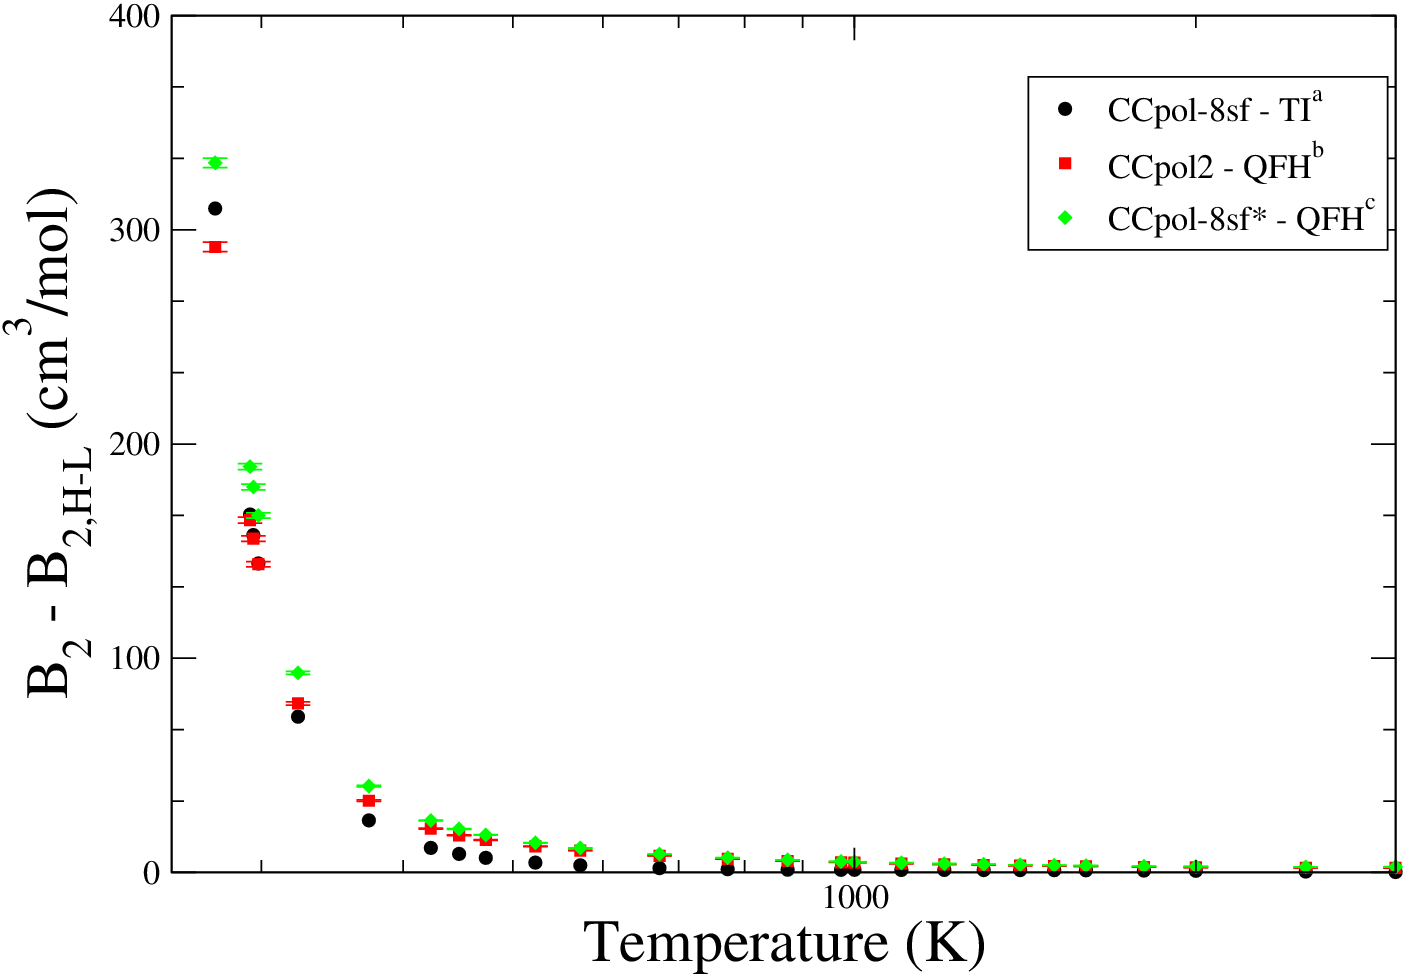
\includegraphics[width=10cm,keepaspectratio]{Chapter-7/Figures/B2SCAll.png}
            \caption{Comparison of the semi-classical second virial coefficient of water for various models including quantum effects, with the experiment based Harvey - Lemmon correlation \cite{Harvey2004} denoted as $B_{2,\text{H-L}}$. $^\text{a}$ - Results from Jankowski et al. \cite{Jankowski2015} using CCpol8sf TI effective potential and vibrational averaging; $^\text{b}$ - Results from Schultz et al. \cite{Schultz2015} using CCpol2 QFH effective potential; $^\text{c}$ - Results from this work using CCpol2 QFH effective potential and vibrationally averaged temperature-dependent geometries. Error bars where shown represent one standard deviation of the mean (68\% confidence interval).}
            \label{fig:B2SC-comparison}
        \end{figure}

        The primary concern of ours lies in the definition of the CCpol-8sf* potential (Eq. \eqref{eq:ccpol8sf*}). The argument made by Jankowski et al. \cite{Jankowski2015} that the definition of hybrid surfaces is made possible only if two (viz., the rigid and the flexible) potentials have been derived using the same ground-state monomer geometries, which is not the case in our calculations. Also, we have ignored embedding of the monomer in the dimer as performed for the flexible potential SAPT-5s'fIR by Jankowski et al. \cite{Jankowski2015}. We assumed that since we are using the ground-state geometries of the rigid potential within the flexible potential, this embedding need not be done. However, this could be significantly affecting the way in which the flexible potential is evaluated.

    \section{Conclusion}
    \label{chap7-sec:conclusion}
        Conclusion here.
    \section{Tabulated Results}
    \label{sec:chap7-tables}
        We report tabulated results for the virial coefficients of water in this section.
        \pgfplotstableset{
            begin table=\begin{longtable},
            end table=\end{longtable},
        }
        \pgfplotstabletypeset[
            columns/temperature/.style={
                string type,
                column name={Temperature(\si{\kelvin})}
            },
            columns/b2sc/.style={
                string type,
                column name=B$_2$(\si{cm^3/mol})
            },
            columns/b3sca/.style={
                string type,
                column name=B$^\text{A}_3$(\si{cm^6/mol^2})
            },
            columns/b3scna/.style={
                string type,
                column name=B$^\text{NA}_3$(\si{cm^6/mol^2})
            },
            columns/b3sctot/.style={
                string type,
                column name=B$^\text{Tot}_3$(\si{cm^6/mol^2})
            },
            every head row/.append style={before row={\caption{Second and third virial coefficients of nitrogen using the hybrid PES defined in Eq. \eqref{eq:ccpol8sf*} and evaluated based on Eq. \eqref{eq:b2ccpol8sf*}. B$^\text{A}_3$ and B$^\text{NA}_3$ represent the additive and non-additive contributions respectively, to the third virial coefficient. B$^\text{Tot}_3$ represents the full third virial coefficient value obtained by summing the additive and non-additive contributions. Values in parantheses are standard uncertainties in the rightmost digit(s).}\label{tab:h2oSCResults}\\\toprule},after row=\midrule\endfirsthead},
            every first row/.append style={before row={\multicolumn{5}{c}{\tablename\ \thetable{} -- Continued from previous page.}\\\toprule},after row=\midrule\endhead},
            every last row/.style={after row=\bottomrule},
        ]{Chapter-7/Tables/SCResultsTable.dat}

